\documentclass[10pt,leqno]{article}

\usepackage[%
  tmargin=1.2in,bmargin=1.2in,%
  lmargin=1.8in,rmargin=1.8in,%
]{geometry}
\usepackage{fancyhdr}
\usepackage{titlesec}
\usepackage{appendix}
\usepackage{microtype}
\usepackage[hyphens]{url}
\usepackage{enumitem}
\usepackage{xspace}
\usepackage{etoolbox}
\usepackage{ifthen}
\usepackage{tikz}
\usepackage{tikz-cd}

\usepackage{amsmath}
\definecolor{darkred}{rgb}{0.5,0.0,0.0}
\usepackage[%
  colorlinks,%
  linkcolor=darkred,%
  citecolor=darkred,%
  urlcolor=darkred,%
]{hyperref}
\usepackage{amsthm,amssymb}
% \usepackage[lining,semibold]{libertine}
% \usepackage{textcomp,stmaryrd}
% \usepackage[libertine,cmintegrals,bigdelims]{newtxmath}
% \useosf
% \usepackage[%
%   cal=boondox, calscaled=0.97,%
%   bb=boondox, bbscaled=0.98,%
% ]{mathalfa}
\usepackage{cleveref}

\frenchspacing
\urlstyle{rm}

\AtBeginDocument{%
  \setlength{\abovedisplayskip}{1.5ex plus 0.3ex minus 0.3ex}%
  \setlength{\abovedisplayshortskip}{1.0ex plus 0.3ex minus 0.3ex}%
  \setlength{\belowdisplayskip}{1.5ex plus 0.3ex minus 0.3ex}%
  \setlength{\belowdisplayshortskip}{1.0ex plus 0.3ex minus 0.3ex}%
}

\let\theoldbibliography\thebibliography
\renewcommand{\thebibliography}[1]{%
  \theoldbibliography{#1}%
  \setlength{\parskip}{0ex}
  \setlength{\itemsep}{0.5ex plus 0.2ex minus 0.2ex}
  \small
}

\pagestyle{fancy}
\renewcommand{\headrulewidth}{0pt}
\renewcommand{\footrulewidth}{0pt}
\fancyhf{}
\fancyfoot[C]{\small\thepage}

\renewcommand{\title}[1]{\newcommand{\thetitle}{#1}}
\renewcommand{\author}[1]{\newcommand{\theauthor}{#1}}
\renewcommand{\date}[1]{\newcommand{\thedate}{#1}}

\renewcommand{\maketitle}{%
  \begin{center}
    {\bfseries\MakeUppercase{%
      \thetitle}}\\[2.5ex]
    {\footnotesize\MakeUppercase{%
      \theauthor}}\\[2.5ex]
    \ifthenelse{\equal{\thedate}{}}{}{%
      \small%
      \setlength{\tabcolsep}{0.2em}%
      \begin{tabular}{rl}
        original: & \thedate \\
        updated: & \today
      \end{tabular}
    }
  \end{center}
  \vspace{2.5ex}
  \thispagestyle{fancy}
}

%%%%%%%%%%%%%%%%%%%%%%%%%%%%%%%%%%%%%%%%%%%%%%%%%%%%%%%%%%%%%%%%%%%%%%

\cspreto{section}{\setcounter{equation}{0}}

\titleformat{\section}{\centering\scshape}{\thesection.}{0.4em}{}
\titlespacing{\section}{0pt}{*4}{*1}
\titleformat{\subsection}{\scshape}{\thesubsection.}{0.4em}{}
\titlespacing{\subsection}{0pt}{*2.5}{*1}

% Display format for equations
\newcommand{\crefeqfmt}[1]{
  \crefformat{#1}{(##2##1##3)}
  \Crefformat{#1}{(##2##1##3)}
  \crefrangeformat{#1}{(##3##1##4--##5##2##6)}
  \Crefrangeformat{#1}{(##3##1##4--##5##2##6)}
  \crefmultiformat{#1}{(##2##1##3}{, ##2##1##3)}{, ##2##1##3}{, ##2##1##3)}
  \Crefmultiformat{#1}{(##2##1##3}{, ##2##1##3)}{, ##2##1##3}{, ##2##1##3)}
  \crefrangemultiformat{#1}{(##3##1##4--##5##2##6}{, ##3##1##4--##5##2##6)}{, ##3##1##4--##5##2##6}{, ##3##1##4--##5##2##6)}
  \Crefrangemultiformat{#1}{(##3##1##4--##5##2##6}{, ##3##1##4--##5##2##6)}{, ##3##1##4--##5##2##6}{, ##3##1##4--##5##2##6)}
}
% Display format for sections
\newcommand{\crefsecfmt}[1]{%
  \crefformat{#1}{\S##2##1##3}
  \Crefformat{#1}{\S##2##1##3}
  \crefrangeformat{#1}{\S\S##3##1##4--##5##2##6}
  \Crefrangeformat{#1}{\S\S##3##1##4--##5##2##6}
  \crefmultiformat{#1}{\S\S##2##1##3}{ and~##2##1##3}{, ##2##1##3}{ and~##2##1##3}
  \Crefmultiformat{#1}{\S\S##2##1##3}{ and~##2##1##3}{, ##2##1##3}{ and~##2##1##3}
  \crefrangemultiformat{#1}{\S\S##3##1##4--##5##2##6}{ and~##3##1##4--##5##2##6}{, ##3##1##4--##5##2##6}{ and~##3##1##4--##5##2##6}
  \Crefrangemultiformat{#1}{\S\S##3##1##4--##5##2##6}{ and~##3##1##4--##5##2##6}{, ##3##1##4--##5##2##6}{ and~##3##1##4--##5##2##6}
}
\crefeqfmt{equation}
\crefeqfmt{enumi}
\crefeqfmt{enumii}
\crefsecfmt{section}
\crefsecfmt{subsection}
\crefsecfmt{appendix}
\crefname{part}{Part}{Parts}
\crefname{chapter}{Chapter}{Chapters}
\crefname{figure}{Figure}{Figures}

\makeatletter

\newcommand{\thmnumfont}{\bfseries}
\newcommand{\thmheadfont}{\bfseries}
\newcommand{\thmnotefont}{\bfseries}
\newcommand{\thmhorizspace}{0.4em}

\def\swappedhead#1#2#3{%
  \thmnumber{\@upn{{\thmnumfont#2}}\@ifnotempty{#1}{.\hspace{0.25em}}}%
  \thmheadfont\thmname{#1}%
  \@ifnotempty{#3}{\ \thmnote{\thmnotefont(#3)}}%
}
\swapnumbers

\newtheoremstyle{block}%
  {2.0ex plus 0.2ex minus 0.1ex}% Space above
  {2.0ex plus 0.2ex minus 0.1ex}% Space below
  {} % Body font
  {} % Indent amount
  {\thmheadfont} % Theorem head font
  {.} % Punctuation after theorem head
  {\thmhorizspace} % Space after theorem head
  {} % Theorem head spec (can be left empty, meaning ‘normal’)

\renewenvironment{proof}[1][Proof]{\par
  \pushQED{\qed}%
  \normalfont%
  \topsep1ex plus 0.2ex minus 0.1ex\relax%
  \labelsep \thmhorizspace\relax%
  \trivlist
  \item[\hskip\labelsep\thmheadfont
    #1\@addpunct{.}]\ignorespaces
}{%
  \popQED\endtrivlist\@endpefalse%
}

\makeatother

\theoremstyle{block}

\newcommand{\defthm}[2]{%
  \newtheorem{#1}[equation]{#2}%
  \crefeqfmt{#1}%
  \newtheorem*{#1*}{#2}%
}

\defthm{algorithm}{Algorithm}
\defthm{conjecture}{Conjecture}
\defthm{construction}{Construction}
\defthm{convention}{Convention}
\defthm{corollary}{Corollary}
\defthm{definition}{Definition}
\defthm{definitions}{Definitions}
\defthm{example}{Example}
\defthm{examples}{Examples}
\defthm{exercise}{Exercise}
\defthm{fact}{Fact}
\defthm{intuition}{Intuition}
\defthm{lemma}{Lemma}
\defthm{notation}{Notation}
\defthm{nothing}{}
\defthm{proposition}{Proposition}
\defthm{question}{Question}
\defthm{remark}{Remark}
\defthm{remarks}{Remarks}
\defthm{situtation}{Situation}
\defthm{theorem}{Theorem}

\setlist{%
  leftmargin=2.5em, parsep=0ex, listparindent=\parindent,
  itemsep=1.0ex, topsep=1.0ex,%
}

\setlist[enumerate, 1]{%
  label=(\alph*),%
  ref=\alph*,%
  widest=d,%
}
\setlist[enumerate, 2]{%
  label=(\roman*),%
  ref=\theenumi.\roman*,%
}
\setlist[itemize, 1]{%
  label=$\vcenter{\hbox{\footnotesize$\bullet$}}$,%
}
\setlist[itemize, 2]{label=--}

%%%%%%%%%%%%%%%%%%%%%%%%%%%%%%%%%%%%%%%%%%%%%%%%%%%%%%%%%%%%%%%%%%%%%%

\makeatletter

\let\ea\expandafter

\newcount\foreachcount

\def\foreachletter#1#2#3{\foreachcount=#1
  \ea\loop\ea\ea\ea#3\@alph\foreachcount
  \advance\foreachcount by 1
  \ifnum\foreachcount<#2\repeat}

\def\foreachLetter#1#2#3{\foreachcount=#1
  \ea\loop\ea\ea\ea#3\@Alph\foreachcount
  \advance\foreachcount by 1
  \ifnum\foreachcount<#2\repeat}

% Roman: \rA is \mathrm{A}
\def\definerm#1{%
  \ea\gdef\csname r#1\endcsname{\ensuremath{\mathrm{#1}}\xspace}}
\foreachLetter{1}{27}{\definerm}
\foreachletter{1}{27}{\definerm}
% Script: \sA is \mathscr{A}
\def\definescr#1{%
  \ea\gdef\csname s#1\endcsname{\ensuremath{\mathscr{#1}}\xspace}}
\foreachLetter{1}{27}{\definescr}
% Calligraphic: \cA is \mathcal{A}
\def\definecal#1{%
  \ea\gdef\csname c#1\endcsname{\ensuremath{\mathcal{#1}}\xspace}}
\foreachLetter{1}{27}{\definecal}
% Bold: \bA is \mathbf{A}
\def\definebold#1{%
  \ea\gdef\csname b#1\endcsname{\ensuremath{\mathbf{#1}}\xspace}}
\foreachLetter{1}{27}{\definebold}
% Blackboard Bold: \lA is \mathbb{A}
\def\definebb#1{%
  \ea\gdef\csname l#1\endcsname{\ensuremath{\mathbb{#1}}\xspace}}
\foreachLetter{1}{27}{\definebb}
% Fraktur: \ka is \mathfrak{a}, \kA is \mathfrak{A}
\def\definefrak#1{%
  \ea\gdef\csname k#1\endcsname{\ensuremath{\mathfrak{#1}}\xspace}}
\foreachletter{1}{27}{\definefrak}
\foreachLetter{1}{27}{\definefrak}
% Sans serif: \iA \is \mathsf{A}
\def\definesf#1{%
  \ea\gdef\csname i#1\endcsname{\ensuremath{\mathsf{#1}}\xspace}}
\foreachletter{1}{6}{\definesf}
\foreachletter{7}{14}{\definesf}
\foreachletter{15}{27}{\definesf}
\foreachLetter{1}{27}{\definesf}
% Bar: \Abar is \overline{A}, \abar is \overline{a}
\def\definebar#1{%
  \ea\gdef\csname #1bar\endcsname{\ensuremath{\overline{#1}}\xspace}}
\foreachLetter{1}{27}{\definebar}
\foreachletter{1}{8}{\definebar} % \hbar is something else!
\foreachletter{9}{15}{\definebar} % \obar is something else!
\foreachletter{16}{27}{\definebar}
% Tilde: \Atil is \widetilde{A}, \atil is \widetilde{a}
\def\definetil#1{%
  \ea\gdef\csname #1til\endcsname{\ensuremath{\widetilde{#1}}\xspace}}
\foreachLetter{1}{27}{\definetil}
\foreachletter{1}{27}{\definetil}
% Hats: \Ahat is \widehat{A}, \ahat is \widehat{a}
\def\definehat#1{%
  \ea\gdef\csname #1hat\endcsname{\ensuremath{\widehat{#1}}\xspace}}
\foreachLetter{1}{27}{\definehat}
\foreachletter{1}{27}{\definehat}
% Checks: \Achk is \widecheck{A}, \achk is \widecheck{a}
\def\definechk#1{%
  \ea\gdef\csname #1chk\endcsname{\ensuremath{\widecheck{#1}}\xspace}}
\foreachLetter{1}{27}{\definechk}
\foreachletter{1}{27}{\definechk}
% Underline: \Aund is \underline{A}, \aund is \underline{a}
\def\defineul#1{%
  \ea\gdef\csname #1und\endcsname{\ensuremath{\underline{#1}}\xspace}}
\foreachLetter{1}{27}{\defineul}
\foreachletter{1}{27}{\defineul}

\makeatother

%%%%%%%%%%%%%%%%%%%%%%%%%%%%%%%%%%%%%%%%%%%%%%%%%%%%%%%%%%%%%%%%%%%%%%

\usetikzlibrary{calc,decorations.pathmorphing,shapes,arrows}
\tikzcdset{
  arrow style=tikz,
  diagrams={>={stealth}},
}

\newcommand{\arrlen}{1em}
\renewcommand{\to}{\mathrel{\tikz[baseline]%
    \draw[>=stealth,->](0,0.5ex)--(\arrlen,0.5ex);}}
\newcommand{\from}{\mathrel{\tikz[baseline]%
    \draw[>=stealth,<-](0,0.5ex)--(\arrlen,0.5ex);}}
\renewcommand{\mapsto}{\mathrel{\tikz[baseline]%
    \draw[>=stealth,|->](0,0.5ex)--(\arrlen,0.5ex);}}
\newcommand{\inj}{\mathrel{\tikz[baseline]%
    \draw[>=stealth,right hook->](0,0.5ex)--(\arrlen,0.5ex);}}
\newcommand{\surj}{\mathrel{\tikz[baseline]%
    \draw[>=stealth,->>](0,0.5ex)--(\arrlen,0.5ex);}}
\newcommand{\fromto}{\mathrel{%
  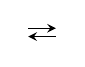
\begin{tikzpicture}[baseline]%
    \draw[>=stealth,<-](0,0.15ex)--(\arrlen,0.15ex);%
    \draw[>=stealth,->](0,0.85ex)--(\arrlen,0.85ex);%
  \end{tikzpicture}}}
\newcommand{\doubto}{\mathrel{%
  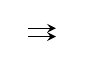
\begin{tikzpicture}[baseline]%
    \draw[>=stealth,->](0,0.15ex)--(\arrlen,0.15ex);%
    \draw[>=stealth,->](0,0.85ex)--(\arrlen,0.85ex);%
  \end{tikzpicture}}}
\newcommand{\lblto}[1]{\mathrel{%
    \begin{tikzpicture}[baseline= {( $ (current bounding box.south) + (0,-0.5ex) $ )}]
      \node[inner sep=.4ex] (a) {\,$\scriptstyle #1$\,};
      \draw[>=stealth,->] (a.south west) -- (a.south east);
    \end{tikzpicture}}}
\newcommand{\isoto}{\lblto{\sim}}

\newcommand{\simpl}[3]{
  \begin{tikzcd}[ampersand replacement=\&, column sep=small]
    #1 \&
    #2 \ar[l, shift right=0.35ex]
       \ar[l, shift left=0.35ex] \&
    #3 \ar[l, shift right=0.70ex]
       \ar[l, shift left=0.70ex]
       \ar[l] \&
    \cdots \ar[l, shift right=0.35ex]
           \ar[l, shift left=0.35ex]
           \ar[l, shift right=1.05ex]
           \ar[l, shift left=1.05ex]
  \end{tikzcd}
}
\newcommand{\cosimpl}[3]{
  \begin{tikzcd}[ampersand replacement=\&, column sep=small]
    #1 \ar[r, shift right=0.35ex]
       \ar[r, shift left=0.35ex] \&
    #2 \ar[r, shift right=0.70ex]
       \ar[r, shift left=0.70ex]
       \ar[r] \&
    #3 \ar[r, shift right=0.35ex]
       \ar[r, shift left=0.35ex]
       \ar[r, shift right=1.05ex]
       \ar[r, shift left=1.05ex] \&
    \cdots
  \end{tikzcd}
}

\newcommand{\tto}{\mathrel{\tikz[baseline]%
    \draw[>=stealth,->,double, double distance = 0.3ex](0,0.5ex)--(\arrlen,0.5ex);}}
\newcommand{\doubfrom}{\mathrel{%
  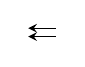
\begin{tikzpicture}[baseline]%
    \draw[>=stealth,<-](0,0.15ex)--(\arrlen,0.15ex);%
    \draw[>=stealth,<-](0,0.85ex)--(\arrlen,0.85ex);%
  \end{tikzpicture}}}
\newcommand{\tripfrom}{\mathrel{%
  
\begin{tikzpicture}[baseline]%
    \draw[>=stealth,<-](0,0.00ex)--(\arrlen,0.00ex);%
    \draw[>=stealth,<-](0,0.50ex)--(\arrlen,0.50ex);%
    \draw[>=stealth,<-](0,1.00ex)--(\arrlen,1.00ex);%
  \end{tikzpicture}}}


\renewcommand{\l}{\left}
\renewcommand{\r}{\right}
\newcommand{\f}{\frac}
\renewcommand{\o}{\overline}
\renewcommand{\u}{\underline}
\newcommand{\til}{\widetilde}
\renewcommand{\hat}{\widehat}
\newcommand{\del}{\partial}
\newcommand{\dash}{\text{-}}
\renewcommand{\c}{\colon}
\newcommand{\lc}{\,:\!}
\newcommand{\ce}{\coloneq}%{\mathrel{:=}}
\newcommand{\ec}{\eqcolon}%{\mathrel{=:}}
\newcommand{\iso}{\simeq}
\newcommand{\dual}{\vee}
\newcommand{\ldb}{\llbracket}
\newcommand{\rdb}{\rrbracket}

\newcommand{\Obj}{\operatorname{Obj}}
\newcommand{\Hom}{\operatorname{Hom}}
\newcommand{\Map}{\operatorname{Map}}
\newcommand{\Fun}{\operatorname{Fun}}
\newcommand{\Aut}{\operatorname{Aut}}
\newcommand{\Iso}{\operatorname{Iso}}
\renewcommand{\id}{\mathrm{id}}
\renewcommand{\im}{\operatorname{im}}
\newcommand{\op}{\mathrm{op}}
\newcommand{\univ}{\mathrm{univ}}
\newcommand{\colim}{\operatorname*{colim}}
\newcommand{\dlim}{\displaystyle\lim}
\newcommand{\dcolim}{\displaystyle\colim}
\newcommand{\Spec}{\operatorname{Spec}}
\newcommand{\Spf}{\operatorname{Spf}}

%%%%%%%%%%%%%%%%%%%%%%%%%%%%%%%%%%%%%%%%%%%%%%%%%%%%%%%%%%%%%%%%%%%%%%


\title{Math 216A Homework 3}
\author{Arpon Raksit}
\date{October 13, 2016}

\numberwithin{block}{section}

%%%%%%%%%%%%%%%%%%%%%%%%%%%%%%%%%%%%%%%%%%%%%%%%%%%%%%%%%%%%%%%%%%%%%%

\begin{document}
\maketitle

\newcommand{\LocRingSpaces}{\mathrm{LocRingSpaces}}
\newcommand{\Rings}{\mathrm{Rings}}

%%%%%%%%%%%%%%%%%%%%%%%%%%%%%%%%%%%%%%%%%%%%%%%%%%%%%%%%%%%%%%%%%%%%%%

\section{Hartshorne exercise  II.2.4}

\begin{nothing}
  \label{global-section}
  Let $X$ be a locally ringed space and $s \in \Gamma(X,\sO_X)$ a global section of its structure sheaf.
  
  \begin{subnotation*}
    For $x \in X$, we will denote the \emph{stalk} of $s$ at $x$ in the local ring $\sO_x$ by $s_x$, and the \emph{value} of $s$ at $x$ in the residue field $\kappa(x) \ce \sO_x/\km_x$ by $s(x)$.
  \end{subnotation*}

  \begin{subnotation*}
    We define $X_s \ce \{x \in X : s(x) \ne 0\}$.
  \end{subnotation*}
  
  \begin{sublemma}
    \label{global-section-nonvanishing-locus}
    \begin{enumerate}[leftmargin=*]
    \item \label{global-section-nonvanishing-locus-open} $X_s$ is an open subset of $X$.
    \item \label{global-section-nonvanishing-locus-invertible} The restriction of $s$ to $X_s$ is invertible in $\Gamma(X_s,\sO_X)$.
    \end{enumerate}
  \end{sublemma}

  \begin{proof}
    Let $x \in X_s$. Then $s(x) \ne 0$ means $s_x \notin \km_x$, and since $\sO_x$ is local this means there exists $t_x \in \sO_x$ such that $s_xt_x = 1$. Thus we can find an open neighborhood $U$ of $x$ and a local section $t \in \Gamma(U,\sO_X)$ with stalk $t_x$ at $x$ such that $s|_Ut = 1 \in \Gamma(U,\sO_X)$. This clearly implies $s(y) \ne 0$ for $y \in U$, i.e. $U \subseteq X_s$. This proves $X_s$ is open.

    We have also proven that we may cover $X_s$ by open subsets $U_i$ which have local sections $t_i \in \Gamma(U_i,\sO_X)$ inverse to (the restrictions of) $s$. But since inverses are unique, these local sections evidently glue to give a well-defined section $t \in \Gamma(X_s,\sO_X)$ inverse to (the restriction of) $s$.
  \end{proof}

  \begin{sublemma}
    \label{global-section-nonvanishing-locus-pullback}
    Let $\pi \c Y \to X$ be a map of locally ringed spaces. Let $\phi \c \Gamma(X,\sO_X) \to \Gamma(Y,\sO_Y)$ denote the pullback of global sections in $\pi$. Then $\pi^{-1}(X_s) = Y_{\phi(s)}$.
  \end{sublemma}

  \begin{proof}
    This is immediate from $\pi$ being a map of \emph{locally} ringed spaces, which implies that $s(\pi(y)) = 0 \iff \phi(s)(y) = 0$.
  \end{proof}
\end{nothing}

\begin{proposition}
  \label{affine-adjunction}
  Let $X$ be a locally ringed space. Let $A$ be a ring. Then the map\footnote{In case it's not clear, here $\LocRingSpaces$ denotes the category of locally ringed spaces and $\Rings$ denotes the category of (commutative, unital) rings.}
  \[
    \alpha \c \Map_\LocRingSpaces(X,\Spec A) \to \Map_\Rings(A, \Gamma(X,\sO_X))
  \]
  given by taking a map $\pi \c X \to \Spec A$ to pullback of global sections in $\pi$ is a bijection.

  \begin{proof}
    Let's write $Y \ce \Spec A$.
    
    We first prove $\alpha$ is injective. Let $\pi \c X \to \Spec A$ be a map of locally ringed spaces, and let $\phi \ce \alpha(\pi) \c A \to \Gamma(X,\sO_X)$ be pullback of global sections. We will show that $\pi$ is uniquely determined by $\phi$.
    
    Let's first consider the map on topological spaces; for $x \in X$ and $s \in A$, we see from \cref{global-section-nonvanishing-locus-pullback} that $x \in \pi^{-1}(Y_s) \iff \phi(s)(x) \ne 0$, or equivalently $\pi(x) \in V(s) \iff \phi(s)(x) = 0$. This implies that $\pi(x)$ must be the prime ideal $\{s \in A : \phi(s)(x) = 0\}$. Hence $\pi$ is determined on topological spaces by $\phi$.

    We now consider the map on structure sheaves $\pi^\sharp \c \sO_Y \to \pi_*\sO_X$. It suffices to show that the map is determined by $\phi$ over the distinguished basic opens $Y_s = D(s)$ for $s \in A$. By \cref{global-section-nonvanishing-locus-pullback} we have $\pi^{-1}(Y_s) = X_{\phi(s)}$. Since $\pi^\sharp$ is a map of sheaves, the diagram
    \[
      \begin{tikzcd}
        \Gamma(Y,\sO_Y) \ar[r, "\pi^\sharp"] \ar[d] &
        \Gamma(X,\sO_X) \ar[d] \\
        \Gamma(Y_s,\sO_Y) \ar[r, "\pi^\sharp"] &
        \Gamma(X_{\phi(s)},\sO_X)
      \end{tikzcd}
    \]
    must commute (where the vertical maps are restriction). But now recall the construction of $\Spec A$: the left map is isomorphic to the localization map $A \to A_s$. By the universal property of localization it follows that the bottom map is determined uniquely by the top map, which is $\phi$. This completes the proof that $\alpha$ is injective.

    We now prove surjectivity, taking cue for our construction from the argument for injectivity. Suppose given a map of rings $\phi \c A \to \Gamma(X,\sO_X)$. We define a map of sets $\pi \c X \to \Spec A$ by setting
    \[
      \pi(x) \ce \{s \in A \c \phi(s)(x) = 0 \in \kappa(x)\}
    \]
    (it's easy to see this is a prime ideal in $A$). For $s \in A$ we have immediately from the definitions that $\pi^{-1}(D(s)) = X_{\phi(s)}$, which is open by \cref{global-section-nonvanishing-locus}\cref{global-section-nonvanishing-locus-open}; since $\{D(s)\}_{s \in S}$ form a base of $\Spec A$, this implies $\pi$ is in fact continuous.

    Now, again writing $Y \ce \Spec A$, we must define a (local) map of sheaves $\pi^\sharp \c \sO_Y \to \pi_*\sO_X$. It suffices to do so on the distinguished base of opens $\{D(s)\}_{s \in A}$ of $Y$ (in a consistent fashion). Globally, i.e. on $D(1) = Y$, we define $\pi^\sharp \c A = \Gamma(Y,\sO_Y) \to \Gamma(X,\sO_X)$ to be $\phi$; thus, when we've finished constructing the map, we'll have $\alpha(\pi) = \phi$, and hence have proven surjectivity. For each basic open $D(s) = Y_s$ we have from the above that $\pi^{-1}(Y_s) = X_{\phi(s)}$; by \cref{global-section-nonvanishing-locus}\cref{global-section-nonvanishing-locus-invertible} the restriction of $\phi(s)$ to $X_{\phi(s)}$ is invertible. Since $\Gamma(Y,\sO_Y) \to \Gamma(Y_s,\sO_Y)$ is isomorphic to the localization map $A \to A_s$, it follows that there is a unique map $\phi_s$ making the diagram
    \[
      \begin{tikzcd}
        \Gamma(Y,\sO_Y) \ar[r, "\phi"] \ar[d] &
        \Gamma(X,\sO_X) \ar[d] \\
        \Gamma(Y_s,\sO_Y) \ar[r, "\phi_s"] &
        \Gamma(X_{\phi(s)},\sO_X)
      \end{tikzcd}
    \]
    commute; we define $\pi^\sharp$ on $Y_s$ to be $\phi_s$. It is immediate from this construction that whenever $Y_t \subseteq Y_s$ the diagram
    \[
      \begin{tikzcd}
        \Gamma(Y_s,\sO_Y) \ar[r, "\phi_s"] \ar[d] &
        \Gamma(X_{\phi(s)},\sO_X) \ar[d] \\
        \Gamma(Y_t,\sO_Y) \ar[r, "\phi_t"] &
        \Gamma(X_{\phi(t)},\sO_X)
      \end{tikzcd}
    \]
    commutes. Hence $\pi^\sharp$ is a well-defined map of sheaves.
    
    Finally, for $x \in X$, we see from the above construction that the induced map on stalks $\pi^\sharp \c A_{\pi(x)} \iso \sO_{\pi(x)} \to \sO_x$ is the localization of the composite $A \to \Gamma(X,\sO_X) \to \sO_x$ at the prime ideal $\pi(x)$. By definition, $\pi(x)$ is the preimage of the maximal ideal $\km_x \subseteq \sO_{\pi(x)}$, and hence this map on stalks is local. Thus $\pi^\sharp$ is a map of locally ringed spaces, finishing the proof.
  \end{proof}

  \begin{subremark}
    \label{affine-adjunction-affine-case}
    Suppose we take $X$ to be an affine scheme $\Spec B$ in the above. Then from the construction of the proof we see that $\alpha^{-1}$ is given precisely by applying the functor $\Spec$.
  \end{subremark}

  \begin{subcorollary}
    \label{affine-adjunction-unit}
    For any locally ringed space $X$, there is a natural map of locally ringed spaces $\eta \c X \to \Spec \Gamma(X,\sO_X)$, which is an isomorphism if and only if $X$ is an affine scheme.

    \begin{proof}
      The map $\eta$ corresponds to the identity map of rings $\Gamma(X,\sO_X) \to \Gamma(X,\sO_X)$ under the bijection $\alpha^{-1}$ of \cref{affine-adjunction}. If $\eta$ is an isomorphism then $X \iso \Spec \Gamma(X,\sO_X)$ is tautologically an affine scheme. The converse, that $\eta$ is an isomorphism if $X$ is affine, follows from \cref{affine-adjunction-affine-case}.
    \end{proof}
  \end{subcorollary}
\end{proposition}

%%%%%%%%%%%%%%%%%%%%%%%%%%%%%%%%%%%%%%%%%%%%%%%%%%%%%%%%%%%%%%%%%%%%%%

\end{document}
